\chapter{Experiments}\label{experiments}
In this section I present experiments on text classification over collected datasets. The main \textbf{target} dataset for evaluations is BABE, due to its high quality and properties.

Because of novelty of the CWNC I also perform a baseline evaluation on this dataset, but furthermore it is not tuned anymore, nor evaluated.
I follow the current standard approaches and use pretrained transformers for further pretraining and fine-tuning. 

A brief summary of the models tested can be found in the following:




\subsection{Czech monolingual models}
\begin{itemize}
    \item \textbf{RobeCzech} \cite{strakarobeczech} - RoBERTa-based model with 125M parameters. Just as its original counterpart, it is trained with \gls{mlm} task, on 4,917M tokens of Czech corpora.
    \item \textbf{Czert} \cite{sido-etal-2021-czert} - BERT-based model with 110M parameters, trained with \gls{nsp} tasks. All Together trained on 37GB of text. 
    \item \textbf{FERNET-C5} \cite{lehevcka2021comparison} - BERT-based model trained with the \gls{mlm} and \gls{nsp} task on 93GB of text from the Common Crawl project.
    \item \textbf{FERNET-News} \cite{lehevcka2021comparison} - RoBERTa-based model trained with \gls{mlm} task on 20GB of Czech News text.
\end{itemize}






\subsection{Multi-lingual models}
\begin{itemize}
    \item \textbf{SlavicBert} \cite{arkhipov2019tuning} - BERT-based model with 179M parameters, trained on four languages: Russian, Bulgarian, Czech, and Polish. The model is trained on all 4 languages at once. The model is not trained from scratch, but it is a fine-tuned version of mBERT.
    \item \textbf{mBERT} - BERT-based model with 179M parameters trained on corpora of 104 languages, Czech included, with MLM task.
\end{itemize}





\section{On Instability of fine-tuning}
bla bla. Cross validace , ukazalo 10x menší variance. -> 10fold cross validace
In turned out that different initializations perform differently on different splits. Therefore increasing number of folds in cross validation reduced the variance 10 times.



\section{Experimental setup}
All models are fetched, trained, and evaluated using the HuggingFace API. The maximum sequence length is set to 128 tokens. All the parameters can be seen in the Appendix.
Everything is evaluated using 10-fold cross-validation. The evaluation metric for all experiments is F1 score with macro averaging\footnote{The score is averaged over all (2) classes.}. 

A small portion (15\%) of the target dataset is left aside as a \textbf{test set} at the beginning and used only for the final evaluation to ensure that there are no test data leaks into training procedure.

All training has been done on a RCI cluster node with 4 x NVIDIA Tesla V100 with 32GB GPU graphic memory.




 \section{Baseline setup}
 As a baseline, all Czech models are fine-tuned on BABE and evaluated using 10-fold stratified cross-validation. Used hyperparameters are the same as those used by the authors of the BABE \cite{Spinde2021MBIC}. However, the authors used early stopping together with cross-validation and used the validation split inside CV to early stop, which allows the model to "see" the test during the tuning, before the evaluation. 
 
 Using early stopping would require another split for validation, but at this point the size of the training data is already shrinked significantly. Hence I did not use early stopping with CV at all and fixed the number of epochs to 3, as authors of BERT suggest \cite{devlin2019bert} . 
 All other hyperaparemeters remained unchanged. AdamW optimizer is used with an initial learning rate 5e-5 and batch size is 64.
 
 Baseline evaluation of all the Czech models used can be seen in table \ref{table:3}. The final F1 score is averaged across all folds. For further experiments and tuning. For further tuning the best model, \textbf{FERNET-C5} is chosen.
 

 
 \begin{table}
\makebox[\textwidth][c]{
\begin{ctucolortab}
\begin{tabular}{c||c|c|c|c|c|c}
 \textbf{target}\textbackslash \textbf{models} & \textbf{Czert} & \textbf{RobeCzech} & \textbf{mBERT} & \textbf{FERNET-C5} & \textbf{FERNET-News} & \textbf{SlavicBERT}\\
 \hline
 \hline
 \textbf{BABE} & 0.739 & 0.773 & 0.743 & \textbf{0.78} & 0.644 & 0.762 \\
 \hline
 \textbf{CWNC} & 0.726 & \textbf{0.758} & 0.734 & 0.689 & 0.602 & 0.729 \\
\end{tabular}
\end{ctucolortab}
\caption{F1 scores of baseline fine-tuning. Best scores for each dataset are highlighted.}
\label{table:3}
}
\end{table}

 
 
 
 
 
 \section{Hyperparameter tuning}
I restricted the search space only to the combinations of:
 \begin{itemize}
     \item \textbf{Batch size} $\in \{16,32\}$
     \item \textbf{Learning rate} $\in $ \{2e-5,3e-5,5e-5\}
     \item \textbf{Epochs} $\in \{2,3,4\}$
 \end{itemize}
 
 As the authors of the original BERT paper suggest.  After running the grid search, the overall best parameters were:
 \begin{center}
      \{learning\_rate = 3e-5,batch\_size = 32, epochs=3\}
 \end{center}
 
 Model with the best parameters achieved 0.784 F1 score ($\sim$0.4\% improvement against baseline).


 
 
  \begin{table}
\makebox[\textwidth][c]{
\begin{ctucolortab}
\begin{tabular}{c||c|c|c|c|c|c|}
  & \textbf{baseline} & \textbf{SUBJ} & \textbf{WIKI} & \textbf{MB} & \textbf{WNC} & \textbf{ALL}\\
 \hline
 \hline
 \textbf{Pretraining + Finetuning} & 0.7835 & 0.7875 & 0.7797 & 0.7702 & 0.7825 & \textbf{0.7878} \\
 \hline
 \textbf{Pretraining + Evaluating} & - & 0.5542 & 0.6344 & 0.4631 & \textbf{0.6697} & 0.6423 \\
\end{tabular}
\end{ctucolortab}
\caption{F1 scores of effects of pretraining on different dataset combinations.}
\label{table:4}
}
\end{table}

 \section{Combining Datasets}
This section is dedicated to the study of the influence of pre-training combination of datasets. Trying all combinations would result in training of 128 models, which is obviously infeasible. Therefore, I decided to pretrain on 5 combinations with regards to the bias information:
\begin{itemize}
    \item \textbf{SUBJ} - is a combination of SUBJ and MPQA dataset, which both focus on explicit subjective bias.
    \item \textbf{MB} - is a combination of NJNJ,UA-crisis and BASIL dataset which are all from the media bias family.
    \item \textbf{WIKI} - are all datasets gather from wikipedia, with respect to NPOV violations. It consists of CW-hard, WikiBias and CWNC.
    \item \textbf{ALL} - This one is simply combination of all datasets except the WNC.
    \item \textbf{WNC} - WNC is almost 90\% of all data, I therefore perform experiments on this dataset seperately.
\end{itemize}
 
While pretraining, small validation set was used for each combination to decide the optimal number of epochs for pretraining. Convergence of validation losses can be seen in figure \ref{fig:all_losses}.
\begin{figure}
  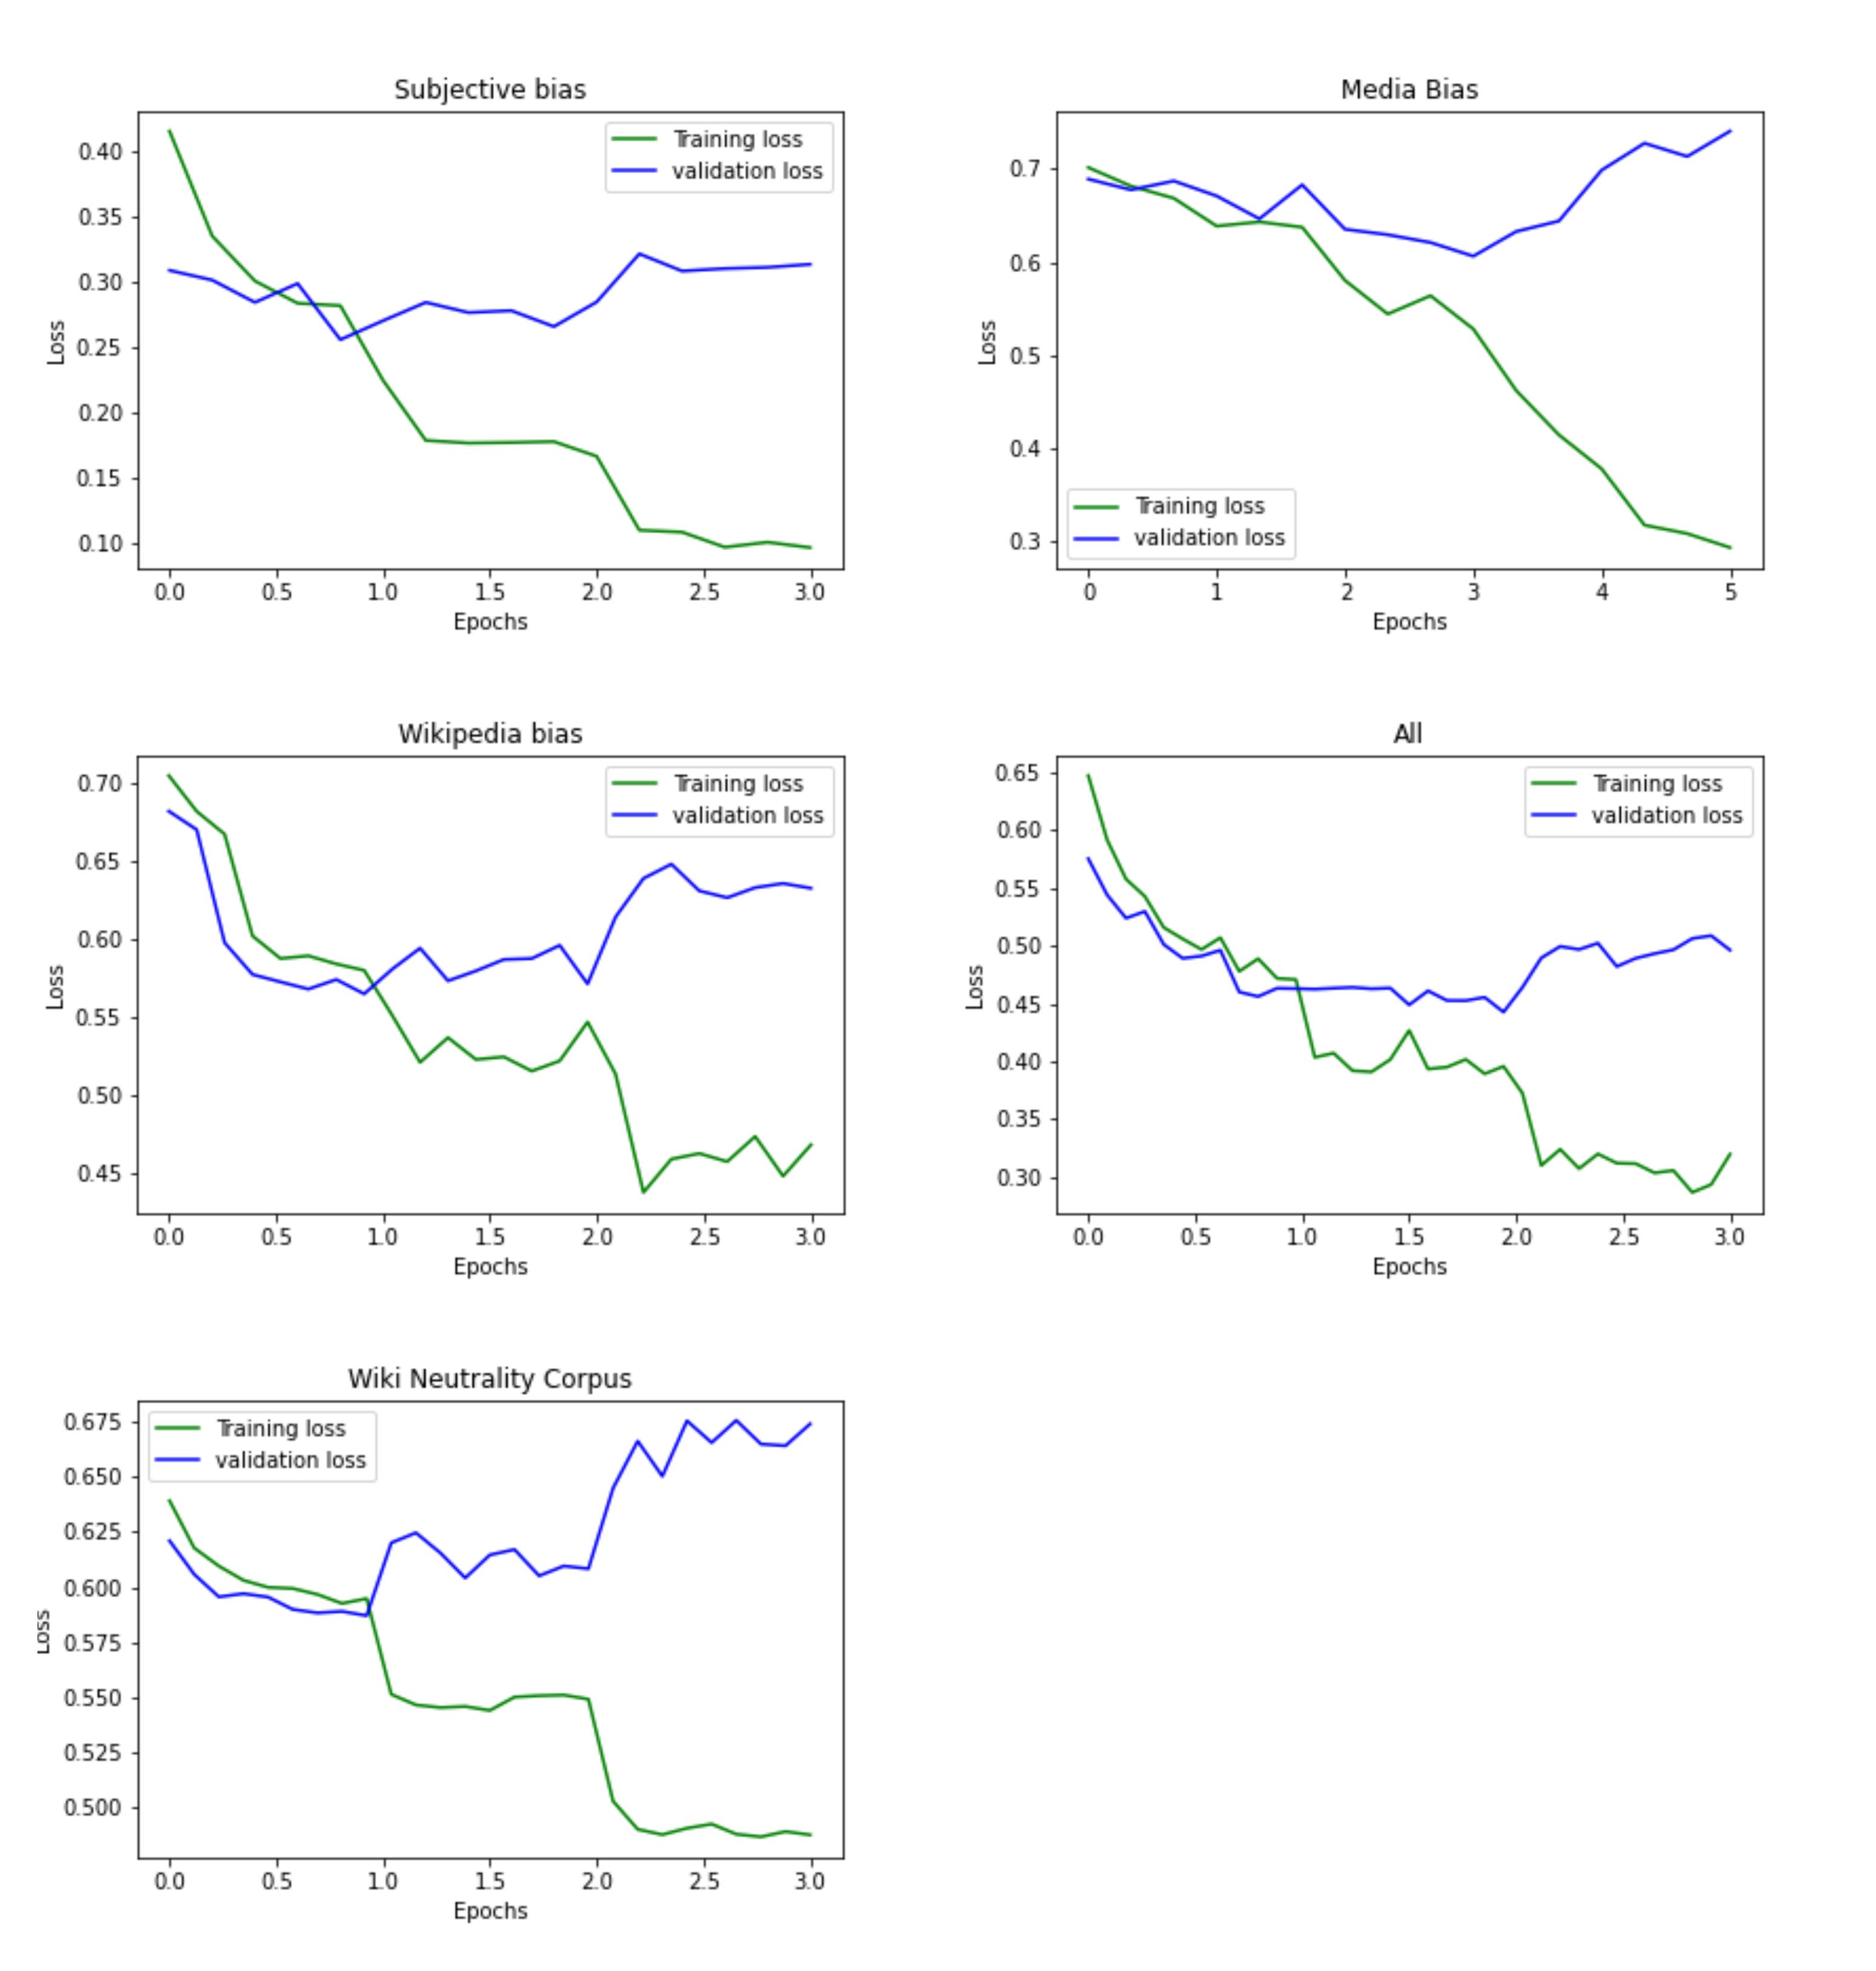
\includegraphics[scale=0.5]{my_modules/multimedia/all_losses.png}
  \caption{Convergence of validation loss over different dataset combinations}
  \label{fig:all_losses}
\end{figure}

Furhermore, I also evaluated pretrained models on babe without fine-tuniing. All results can be seen in \ref{table:4}
The best model out of box was trained on WNC. bla bla All best, however subj good, and subj biggest nad all is mostly subj, mb very bad. wiki bad. interesting subj cant go brr. why because subj is trivial it can help mb with trivials but cant go further. wiki is somewhat balance between triv and hard.

\section{Final evaluation and training}
Final model has been trained with optimal parameters and pretrained on all datasets combined. It achieved F1 score of \textbf{0.804} on a test set. Then for a final model used for inference, the whole dataset has been used.

\section{Conclusion}
The final score on test set is not representative, because of its size. For better evaluation a nested cross-validation should be used. However, the computational demand would be too large. 

A full study with more models could be performed, but that would require enormous umber of trained models. Essentially these results show that there was a very little gain over the baseline (\textbf{+0.7\%}). I suppose that to boost hte performance, novel dataset focused solely on Czech media bias is needed.


  

\section{Inference on Czech News Samples}
\begin{itemize}
    \item Analysis and statistics
    \item Few words Article level
\end{itemize}


%\section{LIME analysis and demo}
%\section{Multi-Task learning approach}\label{mtl}